
%%%%%%%%%%%%%%%%%%%%%%%%%%%%%%%%%%%%%%%%%%%%%%%%%%%%%%%%%%%%%%%%%%%%%
%% This is a (brief) model paper using the achemso class
%% The document class accepts keyval options, which should include
%% the target journal and optionally the manuscript type.
%%%%%%%%%%%%%%%%%%%%%%%%%%%%%%%%%%%%%%%%%%%%%%%%%%%%%%%%%%%%%%%%%%%%%
\documentclass[journal=jacsat,manuscript=article]{achemso}

%%%%%%%%%%%%%%%%%%%%%%%%%%%%%%%%%%%%%%%%%%%%%%%%%%%%%%%%%%%%%%%%%%%%%
%% Place any additional packages needed here.  Only include packages
%% which are essential, to avoid problems later. Do NOT use any
%% packages which require e-TeX (for example etoolbox): the e-TeX
%% extensions are not currently available on the ACS conversion
%% servers.
%%%%%%%%%%%%%%%%%%%%%%%%%%%%%%%%%%%%%%%%%%%%%%%%%%%%%%%%%%%%%%%%%%%%%
\usepackage[version=3]{mhchem} % Formula subscripts using \ce{}
\usepackage[T1]{fontenc}       % Use modern font encodings

%%%%%%%%%%%%%%%%%%%%%%%%%%%%%%%%%%%%%%%%%%%%%%%%%%%%%%%%%%%%%%%%%%%%%
%% If issues arise when submitting your manuscript, you may want to
%% un-comment the next line.  This provides information on the
%% version of every file you have used.
%%%%%%%%%%%%%%%%%%%%%%%%%%%%%%%%%%%%%%%%%%%%%%%%%%%%%%%%%%%%%%%%%%%%%
%%\listfiles

%%%%%%%%%%%%%%%%%%%%%%%%%%%%%%%%%%%%%%%%%%%%%%%%%%%%%%%%%%%%%%%%%%%%%
%% Place any additional macros here.  Please use \newcommand* where
%% possible, and avoid layout-changing macros (which are not used
%% when typesetting).
%%%%%%%%%%%%%%%%%%%%%%%%%%%%%%%%%%%%%%%%%%%%%%%%%%%%%%%%%%%%%%%%%%%%%
\newcommand*\mycommand[1]{\texttt{\emph{#1}}}

%%%%%%%%%%%%%%%%%%%%%%%%%%%%%%%%%%%%%%%%%%%%%%%%%%%%%%%%%%%%%%%%%%%%%
%% Meta-data block
%% ---------------
%% Each author should be given as a separate \author command.
%%
%% Corresponding authors should have an e-mail given after the author
%% name as an \email command. Phone and fax numbers can be given
%% using \phone and \fax, respectively; this information is optional.
%%
%% The affiliation of authors is given after the authors; each
%% \affiliation command applies to all preceding authors not already
%% assigned an affiliation.
%%
%% The affiliation takes an option argument for the short name.  This
%% will typically be something like "University of Somewhere".
%%
%% The \altaffiliation macro should be used for new address, etc.
%% On the other hand, \alsoaffiliation is used on a per author basis
%% when authors are associated with multiple institutions.
%%%%%%%%%%%%%%%%%%%%%%%%%%%%%%%%%%%%%%%%%%%%%%%%%%%%%%%%%%%%%%%%%%%%%
\author{Robert O. Ness}
\email{nessr@purdue.edu}
\affiliation[Purdue University]{Department of Statistics, Purdue University, West Lafayette}
\author{Karen Sachs}
\affiliation[Stanford University]{School of Medicine, Stanford University, Palo Alto}
\email{karens1@stanford.edu}
\author{Olga Vitek}
\email{o.vitek@neu.edu}
\affiliation[Northeastern University]{College of Science, College of Computer and Information Science, Northeastern University, Palo Alto}


%%%%%%%%%%%%%%%%%%%%%%%%%%%%%%%%%%%%%%%%%%%%%%%%%%%%%%%%%%%%%%%%%%%%%
%% The document title should be given as usual. Some journals require
%% a running title from the author: this should be supplied as an
%% optional argument to \title.
%%%%%%%%%%%%%%%%%%%%%%%%%%%%%%%%%%%%%%%%%%%%%%%%%%%%%%%%%%%%%%%%%%%%%
\title[]
  {From Correlation to Causality: Statistical approaches to learning regulatory relationships from Large-scale Omics Experiments}

%%%%%%%%%%%%%%%%%%%%%%%%%%%%%%%%%%%%%%%%%%%%%%%%%%%%%%%%%%%%%%%%%%%%%
%% Some journals require a list of abbreviations or keywords to be
%% supplied. These should be set up here, and will be printed after
%% the title and author information, if needed.
%%%%%%%%%%%%%%%%%%%%%%%%%%%%%%%%%%%%%%%%%%%%%%%%%%%%%%%%%%%%%%%%%%%%%
\abbreviations{IR,NMR,UV}
\keywords{causal inference, big data, causal networks, Bayesian networks}

%%%%%%%%%%%%%%%%%%%%%%%%%%%%%%%%%%%%%%%%%%%%%%%%%%%%%%%%%%%%%%%%%%%%%
%% The manuscript does not need to include \maketitle, which is
%% executed automatically.
%%%%%%%%%%%%%%%%%%%%%%%%%%%%%%%%%%%%%%%%%%%%%%%%%%%%%%%%%%%%%%%%%%%%%
\begin{document}


\begin{abstract}
  Causal inference -- the task of uncovering regulatory relationships between components of biomolecular pathways and networks - is a primary goal of omics experiments in molecular biology studies.  Statistical associations between quantitative measurements can reveal an enticing number of putative causal interactions, but when do such associations reflect the underlying causal biomolecular mechanisms?  The goal of this perspective is to provide suggestions in non-technical terms for causal inference in large scale experiments, resulting from high throughput omics technologies such as MS-based proteomics.  We describe the pitfalls of inference in large datasets, and suggest methods to reliably find causal associations despite these pitfalls.
\end{abstract}

%%%%%%%%%%%%%%%%%%%%%%%%%%%%%%%%%%%%%%%%%%%%%%%%%%%%%%%%%%%%%%%%%%%%%
%% Start the main part of the manuscript here.
%%%%%%%%%%%%%%%%%%%%%%%%%%%%%%%%%%%%%%%%%%%%%%%%%%%%%%%%%%%%%%%%%%%%%
\section{Introduction}
One of the tasks of causal inference methods is to distinguish statistical association resulting from causal relationships from association resulting from indirect relationships. High-throughput omics technologies enable large-scale experiments, with simultaneous measurements of multiple cellular components in a sample. Paradoxically, the large amount of data generated by these experiments make this separation task more difficult, because, when many associations are examined, spurious associations -- associations arising purely from random chance -- may appear as strong as the true associations that result from actual indirect and causal relationships. In other words, large-scale experiments are more prone to hiding true signal and generating spurious associations, leading to increased false positive conclusions that causal relationships are present. This problem can be addressed by improving experimental design and/or refining the biological question. Below, we describe the process of elucidating statistical associations from data and suggest practical approaches for analysis of large scale datasets.


\section{I. Statistical inference of causal relationships: Conditional independence and Interventions}

A biomolecular mechanism creates a causal relationship between molecular species, which may manifest as statistical association between omics measurements of these components. The goal of causal inference performed on these measurements is to elucidate these associations, and determine which of these reflect causal relationships.

\begin{figure}[!tpb]
\centerline{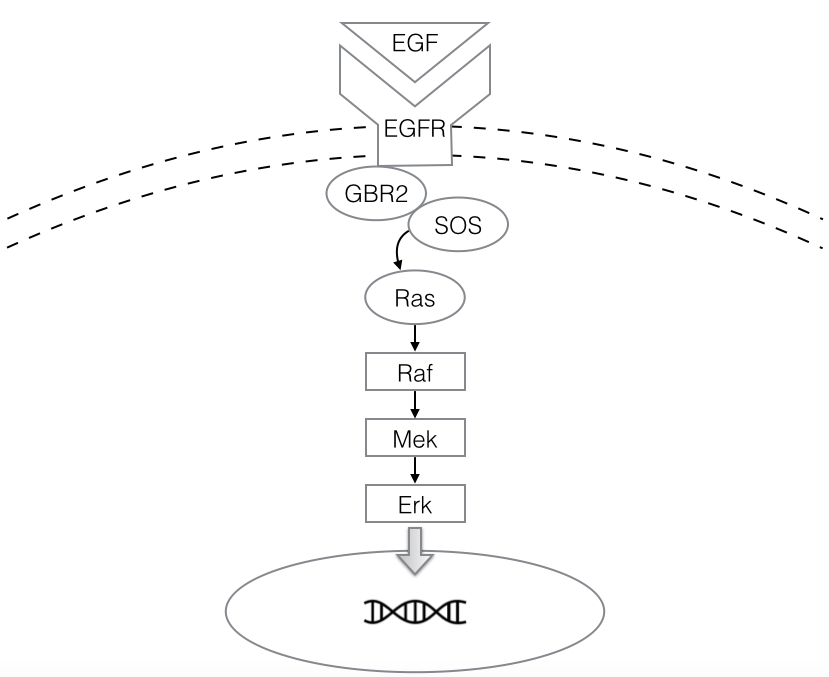
\includegraphics[width=0.5\textwidth]{figs/egfr.png}}
\caption{EGFR MAPK signaling pathway, an example of a pathway containing the phosphorylation cascade from Raf to Mek to Erk.  The binding of ligand EGF to EGFR initiates a signal that leads to the cascade, which leads to gene transcription.  This cascade, a component of several pathways, implies two causal relationships Raf --> MEK, Mek --> Erk.  Raf and Erk have an indirect relationship, through Mek.}
\label{mapk}
\end{figure}

Take for example the MAPK signaling cascade, part of several signaling pathways such as the EGFR MAPK pathway in figure 1. Raf causally affects active Mek levels (via phosphorylation), while Mek causally affects Erk. Imagine these causal relationships were unknown: could they be detected from measurements of these proteins?  

To illustrate causal inference in this context, we use a computational model of the phosphorylation cascade mechanism behind the causal and indirect relationships between Raf, Mek, and Erk.   The Huang-Ferrell computational model of MAPK signaling models the key binding, phosphorylation, and dephosphorylation reactions of the cascade with mass action kinetics, and replicates MAPK key signaling behavior observed in nature.  With this model we simulated an experiment with 100 simultaneous measurements of concentrations of phosphorylated Raf, and doubly phosphorylated Mek and Erk. 

\begin{figure}[!tpb]
\centerline{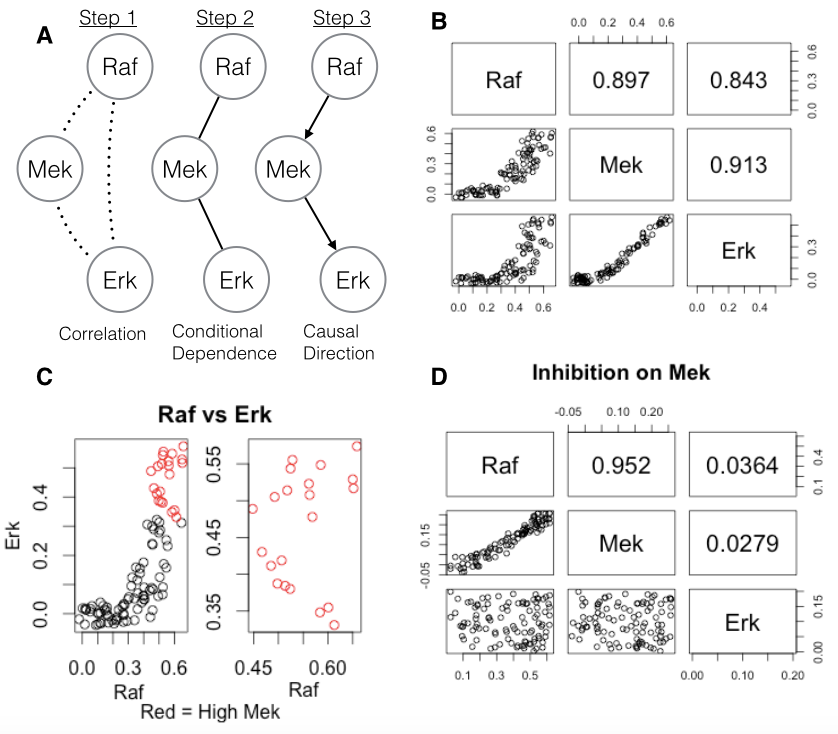
\includegraphics[width=1\textwidth]{figs/mapk.png}}
\caption{A: The causal inference workflow demonstrated on the MAPK cascade.  In step 1, a correlation graph between cascade components Raf, Mek, and Erk is assembled from measurements.  Step 2 reduces the correlation graph a sparse graph of conditional dependencies (Raf--Mek, and Mek--Erk).  Step 3 interrogates this graph to find putative causal relationships (Raf-->Mek, and Mek-->Erk).  While step 1 has little requirements, step 2 requires replicates, and step 3 requires interventions (e.g. inhibitors).  B, C, and D feature an experiment simulated from the Huang-Ferrell computational model of the phosphorylation cascade signaling mechanism.  B: Pairwise plots of concentration values of phosphorylated (doubly phosphorylated for Mek and Erk) forms of each protein, and observed Spearman correlation values.  The Raf -- Erk correlation is high, despite the fact Raf does not directly regulate Erk.  C: Raf values vs Erk, where instances of high Mek values are highlighted in red.  In the right panel of B, Mek is fixed at high levels, and the observed association between Raf and Erk disappear, indicating Raf and Erk are conditionally independent given Mek.  D: After Raf is inhibited, the observed association between Raf and Mek remains while the association between Mek and Erk disappear.  Given Mek is conditionally dependent on Raf and on Erk, the inhibition reveals causal flow from Raf to Mek to Erk.}
\label{mapk}
\end{figure}

Figure 2, panel A demonstrates the causal inference workflow starting with analysis of statistical associations in the data.  Figure 2 panel B shows 2-way plots of the concentration values.  We use Spearman correlation as a measure of association, the top-right half of the plot-matrix displays  the correlation values for each of the 3 pairs.  These high values would meet most reasonable cut-off thresholds for constructing the correlation network in the left part of panel A.  The Raf--Mek and the Mek--Erk correlation edges match the Raf-->Mek, Mek-->Erk known causal edges.  What about the noncausal Raf--Erk edge? Despite the high Raf--Erk correlation, there is no direct causal mechanism between them (aside from the one via Mek, which is already accounted for via the Raf-->Mek and Mek-->Erk edges).  In causal  inference, we can eliminate this "nuisance" edge.  How is this done?

First, some terminology.  When the biological variables  - eg. abundances of specific proteins - have values that move together due to a common biologic mechanism, they are dependent.  Like the mechanism itself, whether or not dependence between two variables exists is typically not known, measures of statistical association (eg  observed Pearson or Spearman correlation, or mutual information) demonstrate empirical evidence of the presence of dependencies between variables.  The problem is that only some  dependencies reflect actual causal relationships, the majority of dependencies reflect indirect relationships One case of dependence through an indirect relationship is when intermediaries exist between an upstream and downstream variable, for example Raf -- Erk dependence comes from their indirect relationship through Mek.  Another such case is one where two variables have a common cause, for example two proteins that don't causally affect one another are dependent if they have the same upstream regulator.  However, when the behavior of the intermediaries or the shared regulators is controlled for, dependency from indirect relationships disappears.  This is called conditional independence.  Causal inference methods attempt to parse causal dependence from indirect dependence by finding empirical evidence of conditional independence. 

Let's see how this applies here, by examining the dependence between Raf and Erk.  Figure 2 panel C compares Raf to Erk, highlighting measurements where Mek values are high (top quartile) in red.  Note that when we subset the data to only the red measurements, in other words when we condition on Mek being high, we can no longer detect the dependence between Raf and Erk.  Based on the causal mechanism, Erk is determined by Mek, so when we fix Mek at a certain level of activity, Erk follows Mek irrespective of Raf levels.  This phenomenon -- wherein the dependence between Raf and Erk disappears upon conditioning on Mek - is evidence that  Raf and Erk are conditionally independent.  Once conditional independence is inferred from the data, the correlation edge arising from Raf--Erk dependence is removed, resulting in the middle graph of Figure 1 panel A.

When we observe all the key variables in a system, variables become conditionally independent of everything except variables with which it shares a direct causal relationship; continuing with the protein signaling example this is a signaling protein's direct regulators, its direct effectors, and other proteins who share its direct effectors.  So after the statistical methods of causal inference pare down a set of observed correlations to a sparse set of putative causal conditional dependence relationships, we rely on interventions to determine the direction of causality.  Figure 2 panel D illustrates the results of an intervention that targeted Mek with an inhibitor.  The concentration of Mek is unaffected but its ability to phosphorylate other proteins is blocked.  After this intervention is introduced, the Raf--Mek relationship is unchanged, while Erk drops to a low level.  From this we can infer that Mek has causal influence on Erk, and since Raf was unaffected by the intervention, that Raf has causal influence on Mek.  With the intervention, we can finally move from the conditional dependence graph in panel A - step 3, to the causal graph in panel A - step 3.

Computational methods for  causal inference follow the workflow  we describe in panel A for Raf-Mek-Erk, scaling it for experiments characterizing multiple intercorrelated variables. They (1) reduce the dense network of pair-wise correlations (or other measures of association) to a sparse network of putative conditional dependencies using empirical evidence of  conditional independence between pairs of variables,  then (2) use information about the interventions included in the experiment to evaluate those conditional dependencies as evidence for potential causal relations.  See Koller-Friedman for a detailed description of these methods and their theoretical underpinnings.

\section{II. Inference with large numbers of variables}

In the context of large-scale experiments, the principal challenge is spurious statistical associations.  These differ from the "nuisance" associations that arise from non-causal indirect albeit actual dependence.  Spurious associations are purely random artifacts of the data, reflecting no actual direct or indirect dependence.

The opportunity for spurious association grows with the number of variables simultaneously measured relative to the number of replicates.  Indeed, the typical large-scale experiments quantify a large number of analytes, and have a small number of replicates.  Measuring more analytes means more analyte pairs where spurious correlation can appear, and having fewer replicates makes it more likely two unrelated analytes will have measurements that align by mere coincidence. The high amount of spurious associations in these experiments confound causal inference methods' task of evaluating true associations to the point of infeasibility.

A simulation illustrates this problem.  The simulation is inspired  by Fan et. al. but is translated to our context. We simulated an experiment, we collect 100 replicates with abundance measurements for 20 proteins.  We then simulate a second experiment where we increase the number of proteins to 500.  In both experiments, each protein in each replicate is assigned a value randomly drawn from a Gaussian distribution.  Because of this, the measurements  for a given protein are completely independent from those of any other, meaning any correlation we find will be completely spurious.   After repeating the experiments 500 times, we plot the histograms of the highest Pearson correlation value found in each case; the light histogram for the 20-protein experiments, the dark histogram for the 500-protein experiments. The 500-protein histogram is to the left of the 20-protein histogram, demonstrating that increasing the number of proteins measured  results in spurious correlations with higher values.  This is a clearly problem when high correlation is used as evidence of a true dependency.


\begin{figure}[!tpb]
\centerline{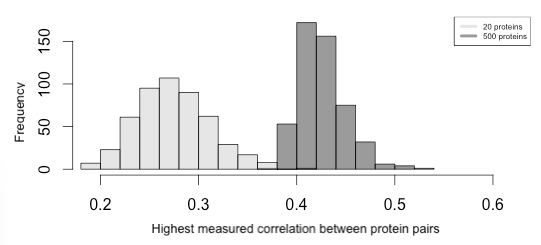
\includegraphics[width=1\textwidth]{figs/spurious_corr.png}}
\caption{In a simulated experiment inspired by Fan et. al., we collect 100 replicates with abundance measurements for 20 proteins.  We then simulate a second experiment where we increase the number of proteins to 500.  In both experiments, each protein in each replicate is assigned a value randomly drawn from a Gaussian distribution.  Because of this, the measurements  for a given protein are completely independent from those of any other, meaning any correlation we find will be completely spurious.   After repeating the experiments 500 times, we plot the histograms of the highest Pearson correlation value found in each case; the light histogram for the 20 protein experiments, the dark histogram for the 500 protein experiments. The 500-protein histogram is to the left of the 20-protein histogram, demonstrating that iIncreasing the number of proteins measured  results in spurious correlations with higher values, which is a problem when high correlation is considered evidence of a true relationship.}
\label{spur_corr}
\end{figure}

The increased incidence of spurious correlation impedes the performance of causal inference methods’ evaluation of conditional independence in the data.  Specifically they result in more false positives in detection of putative causal conditional dependence relationships. To illustrate, we repeated the previous simulation, again starting with 20 proteins with 100 samples each, but this time expanding to only 100 proteins.  Instead of finding the highest  spurious correlation between pairs of proteins, we apply the a causal inference-related algorithm described in Margaritis 2003, which performs a series of conditional independence tests between the sets of proteins.  We obtain a count value for the number of detected conditional dependence relationships.  As before, since we randomly draw protein abundance measurement values from a Gaussian distribution, the values are completely independent, and any conditional dependence relationship reported by this algorithm is a false positive, i.e. it doesn't actually exist in the mechanism that generated the data.  We again repeat these experiments 500 times and generate histograms of the count values in the 20 protein and 100 protein case. 

\begin{figure}[!tpb]
\centerline{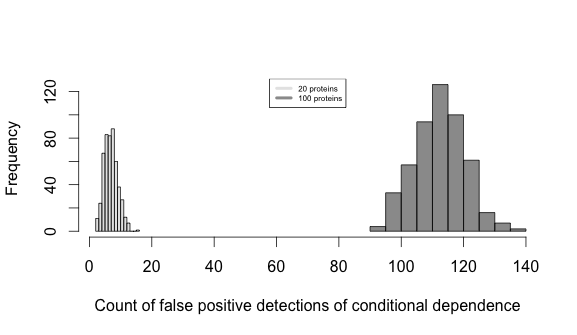
\includegraphics[width=0.5\textwidth]{figs/spurious_dep.png}}
\caption{Results of experiments similar to those demonstrated in figure 2.  We simulate an experiment with 100 replicates of abundance measurements for 20 proteins.  We then simulate a second experiment where we increase the number of proteins to 100.  We apply a causal inference-related algorithm described in Dimitris 2003, which evaluates evidence for conditional independence between sets of proteins, and count the number of pairwise conditional dependence relationships detected by the algorithm.  In both 20-protein and 100-protein experiments, each protein in each replicate was assigned a value randomly drawn from a Gaussian distribution, thus the proteins are completely independent and any detection of a conditional dependence relationship is a false positive, i.e. it doesn't actually exist in the mechanism that generated the data.  We again repeat these experiments 500 times and generate histograms of the conditional dependence detection counts in the 20-protein (light histogram) and 100 protein (dark histogram) case.  The counts of false positive detections in the 20-protein experiments were all less than 20, but in the 100-protein experiments, they were typically greater than 100.  The results demonstrate that increased incidence of spurious correlation resulting from increasing the number of measured proteins, leads to increased false positives in detection of putative causal conditional dependence relationships.}
\label{spur_dep}
\end{figure}

These results demonstrate that the increased incidence of spurious correlation resulting from increasing the number of measured proteins, leads to increased false positives in detection of putative causal conditional dependence relationships. This means that the computational methods for causal inference will fail for the typical large-scale experiment, because when their input data contains a large amount of proteins relative to sample size, they cannot reliably detect the conditional dependence relationships they need to infer causality.

There is a another problem with having the small number of replicates typical of a large scale experiment.  Step 1 of the workflow indicated in figure 2 panel A, evaluating the set of pairwise associations, will work with only a small amount of replicates.  However, the methods for evaluating conditional independence used in step 2 require the statistical degrees of freedom provided by more replicates.  While sparse approaches working with few replicates are available, quality of results decreases drastically as the number of replicates fall.  Note the experiments demonstrated in figure 3 had 100 replicates, a great deal relative to the typical large scale experiments, and still problems emerged.    

Step 3 of the work flow requires interventions to infer causal relationships from evidence of conditional dependence.  Measuring many proteins introduces a  challenge for the step 3 as well. As the number of features grows, the number of interventions needed to fully infer causality grows, and eventually performing a sufficient perturbation experiments becomes infeasible.   We showed with Raf-Mek-Erk example that one intervention was sufficient to infer two causal relationships, and indeed when measuring k variables a set of interventions on < k variables may be sufficient to infer causality.  But along with having too few replicates, the typical large-scale experiment has far too few interventions.  Also, if the step 2 results in too many false positives for conditional dependence, this will adversely affect the results of step 3 regardless of the size of the set of interventions.


\section{III. Approaches for inferring causality from omics experiments}

The problems outlined in section II paint a grim picture for causal learning in large datasets. Fortunately, these can be overcome, and effective causal learning can be a reality for large scale datasets.  We describe best practices  in the Causality Inference in Omics tools below.


\begin{enumerate}
\item \textit{Refine the biological problem}, thus limiting the number of variables.  The length of the list of identified and quantified analytes is not as important as the focus of the investigation and the quantity of measurements on important parts of the system.  If the broader biological system is well-studied, it may be possible design to an experiment that focuses on a specific part of the system of interest, then ask more distinct questions of the data, such as whether a particular edge or pathway is present.  The more specific the question, the less data needed overall to make solid statistical inferences.  
\item \textit{Measure more samples}.  If feasible, high throughput measurements that measure many samples (not just many proteins) provide the statistical power to tell true associations from spurious associations.  This intuition motivates the use of technologies that measure fewer variables but enable measurement of more samples (or gather more data points per sample), for causal modeling.  A related  example is  use of single cell data for inference (e.g. from single cell  mass cytometry), where  many thousands of cells per sample provide ample statistical power. See Sachs et al 2005 for an in depth case study.
\item \textit{Use prior knowledge}, not just from experts but also from noisier sources, to improve the process of searching for conditional independence.  The MAPK pathway for instance, mentioned earlier, is canonical and well established.  The process of inferring causal connections is helped by assuming a priori that such canonical connections exist. This is because knowledge of parts of the underlying regulatory network reduces the remaining number of possible associations, and enables more effective use of data. The number of total associations examined goes down, enabling increased confidence in statistical associations that are found.  Knowledge about canonical causal relationships can be sourced from pathway databases such as KEGG. Another example of prior knowledge is contextual information, such as spatial relations between  signaling proteins in the cell -- causal inference algorithms can be formulated to weigh evidence of conditional dependence differently depending on whether proteins are from the same or different spatial compartments. 
\item \textit{Employ targeted interventions selectively}. Targeted interventions perturb individual components of the system.  An example is small molecule inhibitors which block the causal influence of a specific protein on downstream components.  Since it is usually prohibitive to perturb every target component of a system, it is strategic to prioritize application of targeted interventions to parts of the system that have the most potential for new discoveries.  Selection of these perturbation targets can be based on prior knowledge - e.g. knowledge of which components are crucial players in the system of interest - or they can be applied iteratively, after an initial statistical analysis has revealed areas of the network in which causal inferences are not possible based on existing data.  For instance, a resulting model graph with undirected edges can be inspected to reveal which nodes have potential to reveal the most causality if perturbed.
\item \textit{Consider broad-scale interventions}. Traditionally, experiments characterize a biological response to a particular stimulus, possibly in the context of an inhibitor.  In contrast, broad-scale interventions sacrifice specificity to perturb many features in the system simultaneously.  The advantage of this approach is that it may enable elucidation of  causality across the entire system.  Just as one intervention was sufficient to infer causality between three proteins (Raf, Mek, and Erk), perturbing many things at once creates cascades of causal direction orientation across the broader network.  This includes varying experimental conditions to activate multiple pathways.  For example, signals from endocrine, paracrine, and autocrine ligands elicit various signaling responses in hepatocytes, thus interventions that cover this range of signals gives the best picture of the broader causal network of hepatocyte signaling.  Similarly, interventions that go beyond receptor-level and perturb multiple components of the system bring cascading causal direct orientation deeper into the network.  Although they do not provide specific information about the downstream effects of stimulation,  broad-scale interventions can provide more causal inference bang for your intervention buck.   

\end{enumerate}

\textit{The Causality in Omics Tool List} above provides impactful approaches
that can drastically improve causal inference from omics datasets, by
constraining the inference task, and thus allowing for accurate
statistical inferences. For instance, the task of assessing which of all
the possible KEGG pathways is present in a dataset will be far less
error-prone than the task of assessing which of all possible
combinations of my measured features might form a biological pathway.

How should the tools listed be used? They are most powerful when used in
combination, and in fact the lines between them are somewhat arbitrary
and frequently blurred. For instance, using tool \#1 and tool \#2 in
concert can be thought of as reducing the breadth and increasing the
depth of the investigation. Tools \#4 and \#5 call for use of
interventions, but this task itself is complicated by measuring many
things, since we have more features to expose to intervention. Tool
\#3, prior biological knowledge, can be used to prioritize what to
target with that limited set of interventions.  Causal inference becomes possible when using these tools in combination to design experiments.

\section{Acknowledgement}
We acknowledge the participants of Dagstuhl seminar 15351 "Computational Mass Spectrometry" (December 2015) (http://www.dagstuhl.de/de/programm/kalender/semhp/?semnr=15351) for their contributions to the discussion on computational manuscripts. In particular, we thank the participants of the Correlation vs Causality discussion. We are grateful for the support of Schloss Dagstuhl - Leibniz-Zentrum fur Informatik for supporting the seminar that led to this work.


\end{document}
